% chktex-file 2% chktex-file 29
% chktex-file 13
\documentclass{report}
\usepackage{setspace}
\usepackage[a4paper, total={7in, 10in}]{geometry}
\usepackage[fleqn]{amsmath}
\usepackage{empheq}
\usepackage{amssymb}
\usepackage{amsthm}
\usepackage{gensymb}
\usepackage[fleqn]{cases}
\usepackage{multicol}
\usepackage{color}
\usepackage{stix}
\usepackage{chngcntr}
\usepackage{tikz}
\usepackage{enumitem}
\usepackage{pgfplots}
\usepackage{etoolbox}
\usetikzlibrary{calc,matrix,arrows}
\usetikzlibrary{decorations.pathmorphing,patterns, calligraphy}

\tikzset{
    right angle quadrant/.code={
            \pgfmathsetmacro\quadranta{{1,1,-1,-1}[#1-1]}     % Arrays for selecting quadrant
            \pgfmathsetmacro\quadrantb{{1,-1,-1,1}[#1-1]}},
    right angle quadrant=1, % Make sure it is set, even if not called explicitly
    right angle length/.code={\def\rightanglelength{#1}},   % Length of symbol
    right angle length=2ex, % Make sure it is set...
    right angle symbol/.style n args={3}{
            insert path={
                    let \p0 = ($(#1)!(#3)!(#2)$) in     % Intersection
                    let \p1 = ($(\p0)!\quadranta*\rightanglelength!(#3)$), % Point on base line
                    \p2 = ($(\p0)!\quadrantb*\rightanglelength!(#2)$) in % Point on perpendicular line
                    let \p3 = ($(\p1)+(\p2)-(\p0)$) in  % Corner point of symbol
                    (\p1) -- (\p3) -- (\p2)
                }
        }
}

\counterwithout{equation}{chapter}
\setlength{\columnseprule}{1pt}
\setlength{\columnsep}{24pt}
\setcounter{chapter}{14}
\hfuzz=100pt

\newcommand{\pgfplotsdrawaxis}{\pgfplots@draw@axis}
\makeatother
\pgfplotsset{only axis on top/.style={axis on top=false, after end axis/.code={
                    \pgfplotsset{axis line style=opaque, ticklabel style=opaque, tick style={thick,opaque},
                        grid=none}\pgfplotsdrawaxis}}}

\newtheorem{theorem}{Theorem}

\begin{document}

\newcommand{\sol}[1]{

    \noindent \textbf{Sol.}
}
\newcommand{\prooff}[1]{

    \noindent \textbf{Proof.}
}
\newcommand\m[1]{\begin{pmatrix}#1\end{pmatrix}}
\newcommand\vm[1]{\begin{vmatrix}#1\end{vmatrix}}
\newenvironment{amatrix}[1]{%
    \left(\begin{array}{@{}*{#1}{c}|c@{}}
        }{%
    \end{array}\right)
}
\newenvironment{cequation}{
    \makeatletter
    \setbool{@fleqn}{false}
    \makeatother
    \begin{equation*}
        }{\end{equation*}}

\begin{titlepage}
    \raggedleft{}
    \rule{1pt}{\textheight}
    \hspace{0.02\textwidth}
    \parbox[b]{0.75\textwidth}{

    {\Huge\bfseries Solution Book of \\[0.5\baselineskip] Mathematic}\\[2\baselineskip]
    {\large\textit{Ssnior 2 Part I}}\\[4\baselineskip]
    {\Large\textsc{MELVIN CHIA}}

    \vspace{0.5\textheight}

    {\noindent Written on 9 October 2022}\\[\baselineskip]
    }

\end{titlepage}

\doublespacing{}
\tableofcontents
\singlespacing{}
\newpage

\begin{multicols}{2}

    \chapter{Circle}

    \section{Standard Equation of a Circle}

    The circle is a locus of points in a plane that are equidistant from a fixed
    point called the centre of the circle. The length from the centre to the points
    on the circle is called the radius of the circle.

    \begin{center}
        \begin{tikzpicture}
            \draw[->] (-1,0) -- (5,0) node[right] {$x$};
            \draw[->] (0,-1) -- (0,5) node[above] {$y$};
            \draw (2,2) circle (1.5);
            \filldraw[black] (2,2) circle (0.05);
            \draw[black] (2,1.9) node[below] {\footnotesize$C(h,k)$};
            \filldraw[black] (3.061, 3.061) circle (0.05);
            \draw[black] (2.9, 2.9) node[above right] {\footnotesize$P(x,y)$};
            \draw[black, densely dashed] (2,2) -- (3.061, 3.061);
            \draw[black] (0,0) node[below left] {\footnotesize$O$};
        \end{tikzpicture}
    \end{center}

    The standard equation of a circle is given by
    \begin{cequation}
        (x-h)^2+(y-k)^2=r^2
    \end{cequation}
    where $(h,k)$ is the centre of the circle and $r$ is the radius of the circle.

    If the centre of the circle is at the origin, then the equation of the circle
    is
    \begin{cequation}
        x^2+y^2=r^2\ \ \ \ \ (r>0)
    \end{cequation}

    \subsection{Practice 1}

    \begin{enumerate}
        \item Find the equation of the circle with centre $(3, -1)$ and radius $2$.
        \item Find the equation of the circle with centre $(-2, 9)$ and passing through the
              point $(1, 5)$.
    \end{enumerate}

    \subsection{Exercise 16.1}

    \begin{enumerate}
        \item Find the equation of the circle with centre at the origin and radius $7$.
        \item Find the equation of circle of each of the following description:
              \begin{enumerate}
                  \item Passing through the points $(5, -3)$ and centre at $(2, 1)$.
                  \item Centre at $(3, 2)$ and radius $4$.
                  \item Centre at $(a, b)$ and radius $a+b$.
              \end{enumerate}
        \item Given that the coordinates of two points on the end of the diameter of a circle
              are $(5, -3)$ and $(3, 1)$, find the equation of the circle.
        \item Find the equation of the circle with a diameter connected by the points $(-3,
                  4)$ and $(9, 2)$.
        \item Given two points $P(-2, 2)$ and $Q(4, 6)$, find the equation of the circle wuth
              line $PQ$ as its diameter.
        \item Turn the equation $x^2+y^2-6x+12y+41=0$ into the standard form, and find the
              centre and radius of the circle.
    \end{enumerate}

    \section{General Equation of a Circle}

    Expand the standard equation of a circle, we get
    \begin{cequation}
        x^2+y^2-2hx-2ky+h^2+k^2-r^2=0
    \end{cequation}
    \setlength{\belowdisplayskip}{0pt} \setlength{\belowdisplayshortskip}{0pt}
    \setlength{\abovedisplayskip}{0pt} \setlength{\abovedisplayshortskip}{0pt}
    Let $g=-h$, $f=-k$, $c=h^2+k^2-r^2$, we get the general equation of a circle
    \begin{cequation}
        x^2+y^2+2gx+2fy+c=0
    \end{cequation}
    \begin{flalign*}
        \text{From }c=h^2+k^2-r^2\text{, we have }r^2 & =h^2+k^2-c              & \\
        r                                             & =\sqrt{h^2+k^2-c}       & \\
                                                      & =\sqrt{(-g)^2+(-f)^2-c} & \\
                                                      & =\sqrt{g^2+f^2-c}
    \end{flalign*}
    \setlength{\belowdisplayskip}{10pt} \setlength{\belowdisplayshortskip}{10pt}
    \setlength{\abovedisplayskip}{10pt} \setlength{\abovedisplayshortskip}{10pt}
    \noindent Thus,
    \begin{enumerate}
        \item When $g^2+f^2-c>0$, the image is a real circle with centre $(g,f)$ and radius
              $\sqrt{g^2+f^2-c}$.
        \item When $g^2+f^2-c=0$, the image is point $(g,f)$.
        \item When $g^2+f^2-c<0$, the image does not exist.
    \end{enumerate}

    \subsection{Practice 2}

    \begin{enumerate}
        \item Find the centre and radius of the circle with equation $x^2+y^2-6x-8y+21=0$.
        \item Find the equaton of the circle that passes through the following points:
              \begin{enumerate}
                  \item $A(0, 0)$, $B(2, 0)$, $C(0, -3)$.
                  \item $K(0, 3)$, $L(1, 2)$, $M(2, -1)$.
              \end{enumerate}
        \item Given that the vertices of $\Delta ABC$ are $(1, 2)$, $(2, 5)$ and $(-1, 2)$,
              find the equation of the circumcircle of $\Delta ABC$.
    \end{enumerate}

    \subsection{Exercise 16.2}

    \begin{enumerate}
        \item Find the centre and radius of the circle with the following equation:
              \begin{enumerate}
                  \item $x^2+y^2-64=0$
                  \item $x^2+y^2-4x-8y=44$
                  \item $x^2+y^2-8x=0$
                  \item $9x^2+9y^2+2x-6y-6=0$
                  \item $9x^2+9y^2+2x-6y-6=0$
              \end{enumerate}
        \item Find the equation of the circle that passes through the following points:
              \begin{enumerate}
                  \item $A(1, 1)$, $B(1, -1)$, $C(-2, 1)$
                  \item $F(0, 0)$, $G(3, -3)$, $H(-1, 0)$
                  \item $P(1, 0)$, $Q(0, -3)$, $R(3, 4)$
              \end{enumerate}
        \item A circle passes through point $A(2, 2)$ and $B(5, 3)$ while intersecting the
              line $x+y=4$ at y-axis. Find the equation of the circle.
    \end{enumerate}

    \section{Problems Related to Circles}

    \subsection*{Tangent to a Circle}

    When a straight line $l$ and a circle intersect at a point $P$, the line $l$ is
    called a tangent to the circle, and the point $P$ is called the point of
    contact. The tangent line is perpendicular to the radius at the point of
    contact. That is to say, when the length from the point of tangency to the
    centre of the circle is equal to the radius of the circle, the line is a
    tangent to the circle.

    \begin{center}
        \begin{tikzpicture}
            % draw a circle and its tangent 
            \draw (0, 0) circle (2);
            \draw (2.828, 0) -- (0, -2.828);
            \node at (2.828, 0) [above right] {$l$};
            \filldraw (0, 0) circle (0.05);
            \node at (0, 0) [above left] {$O$};
            \draw (0, 0) -- (1.4142, -1.4142);
            \filldraw (1.4142, -1.4142) circle (0.05);
            \node at (1.4142, -1.4142) [below right] {$P$};
            \node (A) at (0.74, -2.088) {};
            \node (B) at (2.35, -0.478) {};
            \node (P) at (0.84, -0.84) {};
            \draw [black,right angle symbol={A}{B}{P}];

        \end{tikzpicture}
    \end{center}

    \subsection*{Length of a Tangent}

    According to the theorem of length of tangent, the lengths of tangents drawn
    from an external point to a circle are equal.

    \begin{center}
        \begin{tikzpicture}
            % draw a circle and its tangent 
            \draw (0, 0) circle (2);
            \draw (-1, -2.736) -- (4.472, 0);
            \draw (-1, 2.736) -- (4.472, 0);
            \filldraw (0.8894, 1.7889) circle (0.05);
            \node at (0.8894, 1.7889) [above] {$A$};
            \filldraw (0.8894, -1.7889) circle (0.05);
            \node at (0.8894, -1.7889) [below] {$B$};
            \filldraw (0, 0) circle (0.05);
            \node at (0, 0) [left] {$C$};
            \filldraw (4.472, 0) circle (0.05);
            \node at (4.472, 0) [right] {$P$};
            \draw [dashed] (0, 0) -- (4.472, 0);
            \draw [dashed] (0, 0) -- (0.8894, 1.7889);
            \node (A) at (0, 2.236) {};
            \node (B) at (4.472, 0) {};
            \node (P) at (0, 0) {};
            \draw [black,right angle symbol={A}{B}{P}];
        \end{tikzpicture}
    \end{center}

    Let the equation of the circle be $x^2+y^2+2gx+2fy+c=0$, the external point P
    be $(x_1, y_1)$. Connect $PC$ and $CA$, $\angle CPA=90^{\circ}$, the coordinate
    of centre of the circle $C$ be $(-g, -f)$.
    \begin{flalign*}
        \therefore\ CA = \sqrt{g^2+f^2 - c},\ PC = \sqrt{(x_1+g)^2+(y_1+f)^2}
    \end{flalign*}
    \noindent From the Pythagorean theorem,
    \begin{flalign*}
        {PA}^2 & = PC^2 - CA^2                         \\
               & = (x_1+g)^2+(y_1+f)^2 - (g^2+f^2 - c) \\
               & = x_1^2 + y_1^2 + 2gx_1 + 2fy_1 + c
    \end{flalign*}
    Thus, the length of the tangent is given by
    \begin{flalign*}
        PA = \sqrt{x_1^2 + y_1^2 + 2gx_1 + 2fy_1 + c}
    \end{flalign*}
    Note that the coefficient of $x_1$ and $y_1$ in the above equation must be 1.
    \subsection*{Maximum and Minimum Distance of a Point from a Circle}

    Given a circle with centre $C$ and radius $r$ and a point $P$ anywhere on the
    plane,

    When $PC > r$, point $P$ is said to be outside the circle, the maximum distance
    of $P$ from the circle is $M = PC - r$, and the minimum distance of $P$ from
    the circle is $m = PC - r$.
    \begin{center}
        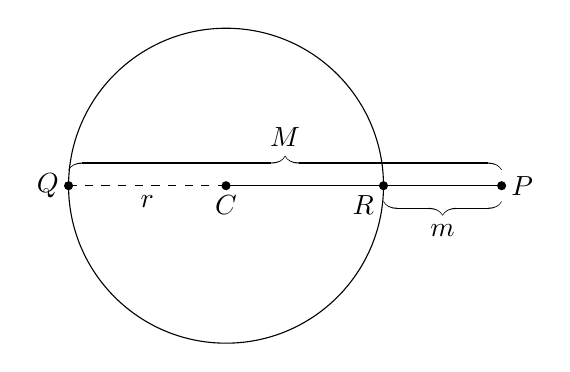
\begin{tikzpicture}
            % draw a circle 
            \draw (0, 0) circle (2);
            \filldraw (0, 0) circle (0.05);
            \node at (0, 0) [below] {$C$};
            \filldraw (2, 0) circle (0.05);
            \node at (2, 0) [below left] {$R$};
            \filldraw (3.5, 0) circle (0.05);
            \node at (3.5, 0) [right] {$P$};
            \filldraw (-2, 0) circle (0.05);
            \node at (-2, 0) [left] {$Q$};
            \draw [dashed] (0, 0) -- (-2, 0) node[pos=0.5,below,black]{$r$};
            \draw (0, 0) -- (3.5, 0);
            \draw [decorate, decoration = {calligraphic brace,amplitude=5pt}] (-2,0.2) --  (3.5,0.2) node[pos=0.5,above=5pt,black]{$M$};
            \draw [decorate, decoration = {calligraphic brace, mirror, amplitude=5pt}] (2,-0.2) --  (3.5,-0.2) node[pos=0.5,below=5pt,black]{$m$};
        \end{tikzpicture}
    \end{center}

    When $PC < r$, point $P$ is said to be inside the circle, the maximum distance
    of $P$ from the circle is $M = PC + r$, and the minimum distance of $P$ from
    the circle is $m = r - PC$.
    \begin{center}
        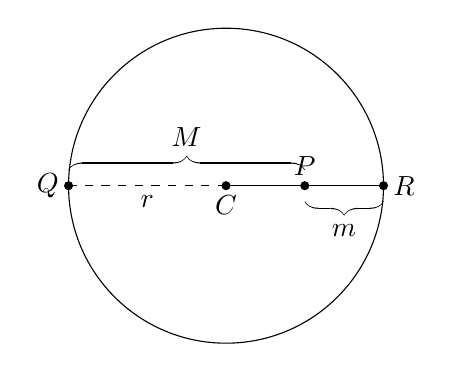
\begin{tikzpicture}
            % draw a circle 
            \draw (0, 0) circle (2);
            \filldraw (0, 0) circle (0.05);
            \node at (0, 0) [below] {$C$};
            \filldraw (2, 0) circle (0.05);
            \node at (2, 0) [right] {$R$};
            \filldraw (1, 0) circle (0.05);
            \node at (1, 0) [above] {$P$};
            \filldraw (-2, 0) circle (0.05);
            \node at (-2, 0) [left] {$Q$};
            \draw [dashed] (0, 0) -- (-2, 0) node[pos=0.5,below,black]{$r$};
            \draw (0, 0) -- (2, 0);
            \draw [decorate, decoration = {calligraphic brace,amplitude=5pt}] (-2,0.2) --  (1,0.2) node[pos=0.5,above=5pt,black]{$M$};
            \draw [decorate, decoration = {calligraphic brace, mirror, amplitude=5pt}] (1,-0.2) --  (2,-0.2) node[pos=0.5,below=5pt,black]{$m$};
        \end{tikzpicture}
    \end{center}

    \subsection{Practice 3}

    \begin{enumerate}
        \item Find the euqaiton of the circle with centre $(3, 4)$ and is tangent to the line
              $yx + 2y - 6 = 0$.
        \item A circle passes through the points $(2, -3$ and $(-2, -5)$, and its centre is
              on the line $x - 2y = 3$. Find the equation of the circle.
        \item A cirle with radius $\sqrt{5}$ and are tangent with the line $x - 2y - 1 = 0$
              at the point $(3, 1)$. Find the equation of the circle.
        \item Prove the following lines are tangent to the following circles:
              \begin{enumerate}
                  \item $3x - y - 5 = 0$, $x^2 + y^2 - 16x + 2y + 25 = 0$
                  \item $2x - y - 1 = 0$, $x^2 + y^2 + 2x - 4y = 0$
              \end{enumerate}
        \item Find the length of the tangent from the point $P(8, 3)$ to the circle $x^2 +
                  y^2 - 8 = 0$.
    \end{enumerate}

    \subsection{Exercise 16.3}

    \begin{enumerate}
        \item Find the equation of the circle that passes through the points $(1, 4)$ and
              $(0, -3)$, and its centre is on the line $x - 2y = 4$.
        \item Find the equation of the circle that passes through the points $(3, 2)$ and
              $(-4, -5)$, and its centre is on the line $3x + y + 6 = 0$.
        \item Find the equation of the circle that passes through the points $A(5, 2)$ and
              $B(-3, 0)$, and its centre is on the y-axis.
        \item Find the equation of the circle with centre at the origin and is tangent to the
              line $3x - 4y + 20 = 0$.
        \item Find the equation of the circle with centre $A(-5, 4)$, and is tangent to the
              x-axis.
        \item Find the equation of the circle with centre $(-4, 2)$, and is tangent to the
              line $3x + 2y = 5$.
        \item Find the equation of the circle that passes through the point $(3, 0)$, and is
              tangent to the line $2x - 3y - 24 = 0$ at point $(3, -6)$.
        \item Given a circle $C_1$ and another circle $C_2: x^2 + y^2 - 4x - 6y + 8 = 0$
              shares the same centre, and $C_1$ is tangent to the line $3x + 4y - 13 = 0$.
              Find the equation of the circle $C_1$.
        \item Prove the following lines are tangent to the following circles:
              \begin{enumerate}
                  \item $6x + 5y - 31 = 0$, $x^2 + y^2 + 4x - 5y - 5 = 0$
                  \item $3x + 1 = 0$, $9x^2 + 9y^2 + 3x + 6y + 1 = 0$
              \end{enumerate}
        \item Find the length of the tangent from the following circles to the following
              circles:
              \begin{enumerate}
                  \item $(-2, 3)$, $x^2 + y^2 - 6x - 2y = 0$
                  \item $(-6, 0)$, $x^2 + y^2 - 6x + 2y + 8 = 0$
                  \item $(2, 2)$, $2x^2 + 2y^2 + 2x + 4y - 3 = 0$
              \end{enumerate}
        \item If the following lines and circles are tengant to each other, find the value of
              $k$:
              \begin{enumerate}
                  \item $4x + 3y - k = 0$, $x^2 + y^2 - 6x + 4y - 12 = 0$
                  \item $x + 3y + k = 0$, $2x^2 + 2y^2 + 12y + 13 = 0$
              \end{enumerate}
        \item Find the maximum and minimum distance of the point $P(-2, 5)$ from the circle
              $x^2 + y^2 - 2x - 2y + 1 = 0$.
        \item Find the maximum and minimum distance of the point $Q(0, 1)$ from the circle
              $x^2 + y^2 - 6x - 10y - 2 = 0$.
        \item Assume that the maximum and minimum distance of the point $R(5, 2)$ from the
              circle $x^2 + y^2 - 4x + 4y - 1 = 0$ are $M$ and $N$ respectively, find the
              product of $M$ and $N$.
    \end{enumerate}

    \section{Revision Exercise 16}

    \begin{enumerate}
        \item Find the euqation of the following circles:
              \begin{enumerate}
                  \item A circle with centre $(1, -1)$ and radius $3$.
                  \item A circle with centre $(2, -3)$ and radius $7$.
              \end{enumerate}
        \item Find the equation of the circle with centre at the origin and passes through
              the point $(2, -1)$.
        \item Find the equation of the circle with centre at $(-5, 6)$ and passes through the
              point $(2, 3)$.
        \item Find the equation of the circle with diameter connecting the points $(2, -5)$
              and $(8, 1)$.
        \item Find the centre and radius of the following circle:
              \begin{enumerate}
                  \item $x^2 + y^2 - 6x + 14y + 50 = 0$
                  \item $x^2 + y^2 + 5x - 2y + 1 = 0$
                  \item $3x^2 + 3y^2 + 6x - 12y + 1 = 0$
                  \item $4x^2 + 4y^2 - 12x + 16y - 7 = 0$
              \end{enumerate}
        \item Find the equation of the circle that passes through the following three points:
              \begin{enumerate}
                  \item $(-1, -1)$, $(-3, 5)$, $(1, 3)$
                  \item $(2, 1)$, $(2, -4)$, $(3, -5)$
                  \item $(0, 0)$, $(0, a)$, $(b, 0)$
              \end{enumerate}
        \item Given the radius of of the circle $x^2 + y^2 - 8x + 10y + c$ is $9$, find the
              value of $c$.
        \item Given two circles $x^2 + y^2 - 2x - 4y - 95 = 0$ and $x^2 + y^2 - 8x - 12y + 48
                  = 0$, find the distance between their centres.
        \item Find the equation of the circle with centre at $(1, -1)$ and is tangent to the
              line $5x - 12y + 9 = 0$.
        \item Find the equation of the circle that passes through the points $(1, -1)$ and
              $(1, 1)$, and is tangent to the line $x - 2 = 0$.
        \item Find the equation of the circle that passes through the points $(6, 4)$ and
              $(1, 7)$, and its centre is on the line $2x - 3y = 6$.
        \item Find the equation of the circle that passes through the points $(-1, 1)$ and
              $(1, 3)$, and its centre is on x-axis.
        \item Find the equation of the circle that is tangent to the line $3x + 4y + 18 = 0$
              at point $(-2, -3)$, and its centre is on the line $x - y = 0$.
        \item If the following lines and circles are tangent to each other, find the value of
              $k$:
              \begin{enumerate}
                  \item $2x - y + k = 0$, $x^2 + y^2 - 1 = 0$
                  \item $2x + 3y + 3\sqrt{13} = 0$, $x^2 + y^2 = k$
                  \item $y = x + k$, $x^2 + y^2 = 9$
              \end{enumerate}
        \item If the circle $x^2 + y^2 - 6y - 4y + k = 0$ is tangent to the x-axis, find the
              value of $k$ and the coordinates of the point of tangency.
        \item Given the coordinates and equations of the following points and circles
              respectively, find the length of the tangent from the point to the circle:
              \begin{enumerate}
                  \item $(1, 6)$, $x^2 + y^2 + 2x - 19 = 0$
                  \item $(2, 4)$, $x^2 + y^2 - 2x + 6y + 9 = 0$
                  \item $(3, 2)$, $2x^2 + 2y^2 + 10x + 11y - 52 = 0$
                  \item $(0, 0)$, $x^2 + y^2 - 2ax + 4ay + 4a^2 = 0$
              \end{enumerate}
        \item Prove that the distance of the tangent from the point $A(3, -4)$ to the circle
              $C_1: x^2 + y^2 - 10x - 7y + 13 = 0$ is equal to the distance of the tangent to
              the circle $C_2: x^2 + y^2 - 10x - 7y + 26 = 0$.
        \item Find the longest and the shortest distance of the point $P(-5, -12)$ to the
              circle $x^2 + y^2 + 8y - 6y = 0$.
        \item Given the equation of circle $x^2 + y^2 + 8y - 6y = 0$.
              \begin{enumerate}
                  \item Find the centre and radius of the circle.
                  \item Prove that $P(-2, 7)$ is on the circle.
                  \item Find the equation of chord of the circle that is split into two equal parts by
                        the point $P(-2, 7)$.
              \end{enumerate}
    \end{enumerate}

\end{multicols}
\end{document}